\documentclass[11pt, oneside]{article}   

\usepackage[english]{babel}
\usepackage{geometry}  
\usepackage{graphicx}      
\usepackage{tabularx}      
\usepackage{amssymb}
\usepackage{amsmath}
\usepackage{booktabs}
\usepackage{hyperref}
\usepackage{achemso}
\usepackage{csquotes}
\usepackage{cleveref}
\usepackage{siunitx}
\usepackage{geometry}
\geometry{left=4cm, right=4cm}

\usepackage[dvipsnames]{xcolor}
\definecolor{tumblue}{rgb}{0,0.396078431372549,0.741176470588235}

\usepackage{xspace}
\usepackage{caption}
\usepackage{subcaption}
\usepackage{authblk} 

\usepackage{sectsty} 
\usepackage[acronym]{glossaries}
\usepackage[sort&compress,numbers,super]{natbib}

\sectionfont{\color{tumblue}\selectfont\sffamily}
\subsectionfont{\color{tumblue}\selectfont\sffamily}
\subsubsectionfont{\color{tumblue}\selectfont\sffamily}
\paragraphfont{\selectfont\sffamily}
\subparagraphfont{\color{gray}\selectfont\sffamily}


\renewcommand*{\Authfont}{\sf}
\renewcommand*{\Affilfont}{\sf}


\definecolor{halfgray}{gray}{0.55}
\renewcommand\labelitemi{\color{halfgray}$\bullet$} 

 
\usepackage{kpfonts}
\usepackage{biolinum}

\clubpenalty = 10000 
\widowpenalty = 10000 
\displaywidowpenalty = 10000


\usepackage{lipsum}
\usepackage[labelfont=bf]{caption}

\newacronym{llm}{LLM}{large language model}
\newacronym{ml}{ML}{machine learning}
\newacronym{agi}{AGI}{artificial general intelligence}
\newacronym{api}{API}{application programming interface}
\newacronym{mcq}{MCQ}{multiple-choice question}
\newacronym{rest}{REST}{Representational State Transfer}
\newacronym{orm}{ORM}{object relational mapping}
\newacronym{dai}{DAI}{daily allowed intake}
\newacronym{ghs}{GHS}{Globally Harmonized System of Classification and Labelling of Chemicals}
\newacronym{who}{WHO}{World Health Organization}
\newacronym{nmr}{NMR}{Nuclear Magnetic Resonance}
\newacronym{helm}{HELM}{Holistic Evaluation of Language Models}
\newacronym{smiles}{SMILES}{Simplified Molecular Input Line-Entry System}
\newacronym{pca}{PCA}{Principal Component Analysis}
\newacronym{iupac}{IUPAC}{International Union of Pure and Applied Chemistry}
\newacronym{json}{JSON}{JavaScript Object Notation}
\usepackage{credits}
\usepackage{orcidlink}
\usepackage{showyourwork}
% \usepackage[backend=biber,style=numeric,citestyle=numeric-comp, sorting=none, url=true, maxbibnames=99]{biblatex}

\title{\textsf{Are frontier models superhuman chemists?}}

% exact order TBD but first three contributed equally? 
\author[1]{Nawaf~Alampara}

\author[1]{Adrian~Mirza~\orcidlink{}}

\author[1]{Sreekanth~Kunchapu~\orcidlink{}}

\author[]{Aswanth~Krishnan}

\author[1]{Mara~Willhelmi}

\author[1]{Macjonathan~Oreke}

\author[]{Benedict~Emoekabu}

\author[5]{Tanya~Gupta}

\author[5]{Philippe~Schwaller~\orcidlink{0000-0003-3046-6576}}

\author[]{Michael Pieler~\orcidlink{0000-0001-9186-7045}}

\author[1,2, 3]{Kevin~Maik~Jablonka~\orcidlink{0000-0003-4894-4660}}
\affil[1]{Laboratory of Organic and Macromolecular Chemistry (IOMC), Friedrich Schiller University Jena, Humboldtstrasse 10, 07743 Jena, Germany}
\affil[2]{Center for Energy and Environmental Chemistry Jena (CEEC Jena), Friedrich Schiller University Jena, Philosophenweg 7a, 07743 Jena, Germany}
\affil[3]{Helmholtz Institute for Polymers in Energy Applications (HIPOLE), Philosophenweg 7a, 07743 Jena, Germany}
\affil[]{\texttt{mail@kjablonka.com}}


\begin{document}
\maketitle

\begin{abstract}
% \lipsum[1]
\end{abstract}

\clearpage

% cite https://link.springer.com/article/10.1038/s41598-024-54936-7 
\section{Introduction}
\Glspl{llm} are frontier \gls{ml} models trained on massive amounts of text to complete sentences. 
While some see in them \enquote{sparks of \gls{agi}},\cite{bubeck2023sparks} others consider them as \enquote{stochasitc parrots}---i.e., systems that only regurgitate what they have been trained on.\cite{bender2021dangers} 

Chemists and materials scientists have quickly caught on the mounting attention given to \glspl{llm}, some even suggesting that \enquote{the future of chemistry is language}.\cite{White_2023} 
This statement is motivated by a growing number of reports that use \glspl{llm} to properties of molecules or materials,\cite{jablonka202314, jablonka2024leveraging, xie2024fine} to optimize reactions\cite{ramos2023bayesian, kristiadi2024sober} or generate materials,\cite{rubungo2023llm, flam2023language, gruver2024fine} extract information,\cite{Patiny_2023, Dagdelen_2024, Zheng_2024, lála2023paperqa, caufield2023structured} or to even build \enquote{autonomous} systems that can physically perform reactions provided a command in natural language.\cite{bran2023chemcrow, Boiko_2023, darvish2024organa} 
The rapid increase in capabilities led to concerns about the potential for dual use of these technologies, e.g., for the design of chemical weapons.\cite{gopal2023releasing, ganguli2022red, Urbina_2022} 
Moreover, the use of these models is now also widespread among students\cite{Intelligent.com_2023} as well as research groups. For some users, misleading information---especially about safety-related aspects---might lead to harmful outcomes. Unfortunately, apart from anecdotal reports there is little evidence on how \glspl{llm} perform compared to experts.

Thus, to better understand what \glspl{llm} can do for chemistry and materials science, and where they might be improved with further developments, a comprehensive analysis is needed. 
For the development of \glspl{llm}, such evaluation is currently mostly performed via standardized benchmarks such as BigBench\cite{srivastava2022beyond} or the LM Eval Harness.\cite{eval-harness} 
The former contains, among 204 tasks, only two tasks classified as \enquote{chemistry related} whereas the latter contains no specific chemistry tasks. 
Due to the lack of widely excepted standard benchmarks, the developers of chemical language models\cite{jablonka2024leveraging, guo2023large, ahmad2022chemberta2, Cai_2024} frequently utilize language-interfaced\cite{dinh2022lift} tabular datasets such as the ones reported in MoleculeNet,\cite{wu2018moleculenet} Therapeutic Data Commons\cite{huang2021therapeutics} or MatBench.\cite{dunn2020benchmarking} 
While those evaluations can measure how well models can make predictions for very specific tasks, they only give a poor measure of how useful those models might be as a chemical assistant. 

While some benchmark based on university entrance exams\cite{Zaki_2024, arora2023llms} or automatic text mining\cite{song2023honeybee, wei2021chemistryqa} have been proposed, also those do not satisfy the following basic criteria chemistry benchmarks should satisfy: 
\begin{itemize}    
    \item \emph{End-to-end automation}. For model development, the evaluations will need to be run many times (e.g., on regular intervals of a training run). 
    Approaches that rely on humans scoring the answers of a system\cite{Schulze_Balhorn_2024, ai4science2023impact} can thus not be used.
    \item \emph{Careful validation by experts}. Manual curation is needed to minimize number of incorrect or unanswerable questions.\cite{northcutt2021pervasive} 
    This is motivated by the observation that many widely used benchmarks are plagued by noisiness.\cite{Frye_2023, Awg} 
    \item \emph{Usable with models that support special treatment of molecules}. Some models such as Galactica\cite{taylor2022galactica} use special tokenization or encoding procedures for molecules or equations. 
    To support this, the benchmark system must encode the semantic meaning of various parts of the question or answer. 
    \item \emph{Usable with black box systems}. Many relevant systems do not provide access to model weights or even just the raw logits. 
    This might be the case because the systems are proprietary or because they involve not only \glspl{llm} but also external tools such as search \glspl{api} or code executors.\cite{schick2024toolformer, karpas2022mrkl, yao2022react} 
    Thus, a benchmark should not assume access to the raw model outputs but be able to operate on text completions.
    \item \emph{Probing capabilities beyond answering of \glspl{mcq}}. In real world chemistry as well as higher-level university education multiple choice question are seldom utilized. 
    Yet, most benchmarking frameworks focus on the \gls{mcq} setting because of the ease of evaluation. Realistic evaluations must measure capabilities beyond the answering of \gls{mcq}.
    \item \emph{Cover a diverse set of topics}. Chemistry, as the \enquote{central science}, bridges multiple disciplines.\cite{Aspuru_Guzik_2018} To even just approximate \enquote{chemistry capabilities} the topics covered by a chemistry benchmark must be very diverse.
\end{itemize}


In this work, we report a novel benchmarking framework, chembench, and use it to reveal limitations of current frontier models for the use in the chemical sciences.
Our benchmark consists of \variable{output/total_number_of_questions.txt}\unskip question answer pairs manually (\variable{output/manually_generated.txt}\unskip) or semi-automatically (\variable{output/automatically_generated.txt}\unskip) compiled from diverse sources. 
It covers a large fraction of the topics taught in undergraduate chemistry curricula at various skill levels and can be used with any system that can return text (i.e., also tool-augmented systems).

To contextualize the scores, we also surveyed more than \variable{output/number_experts.txt}\unskip experts in chemistry (for a total of number of more than \variable{output/number_experts.txt}\unskip) on a subset of the benchmark corpus to be able to compare the performance of current frontier models with the one of humans.
Our results indicate that current frontier models perform \enquote{superhuman} on some aspects of chemistry but in many cases, included safety-related ones, might be very misleading. 


\section{Results}

\subsection{Benchmark dataset}

To compile our benchmark corpus we utilized a broad list of sources (\Cref{sec:curation}), ranging from university exams to semi-automatically generated questions based on curated subsets of data in chemical databases. 
To ensure maximal interoperability, we curated the data in an extended form of the BigBench format. 
This also implies that future baselines can be built on top of our infrastructure as long as they are saved in the same format. 
For quality assurance, all questions have been reviewed by at least one scientist in addition to the original curator.

Importantly, our large pool of questions encompassed a wide range of topics. 
This can be seen, for example, in \Cref{fig:topic_barplot} in which we compare the number of questions in different categories (see \Cref{sec:meth-topic} for details on how we assigned topics). 
By design, a focus of our corpus is on safety-related aspects with a (currently) limited sampling of questions from physical or theoretical chemistry, which might be extended in future work.

\begin{figure}
    \centering
    \includegraphics{figures/question_count_barplot.pdf}
    \caption{\textbf{Number of questions for different topics.} The topics have been assigned using a combination of a rule-based system (mostly based on the source the question has been sampled from) as well as a classifier operating on a word-embedding of the question. The figure shows that not all aspects of chemistry are equally represented in our corpus. The corpus currently focuses on safety-related aspects.}
    \label{fig:topic_barplot}
    \script{plot_statistics.py}
\end{figure}

Importantly, the corpus samples both \gls{mcq} and open-ended questions in a balanced way (). As one might expect, most questions are difficult to read according to the Flesch–Kincaid readability test (\num{57\pm18}). \cite{kincaid1975derivation}


\begin{figure}
    \centering 
    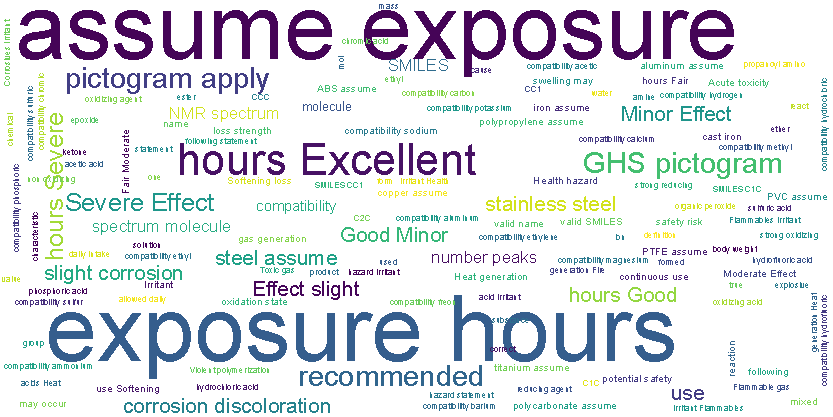
\includegraphics{figures/wordcloud.pdf}
    \caption{\textbf{Co-occurrence graph of entities across questions.}}
    \label{fig:wordcloud}
\end{figure}


\subsection{Model evaluation}


\begin{figure}
    \centering
    %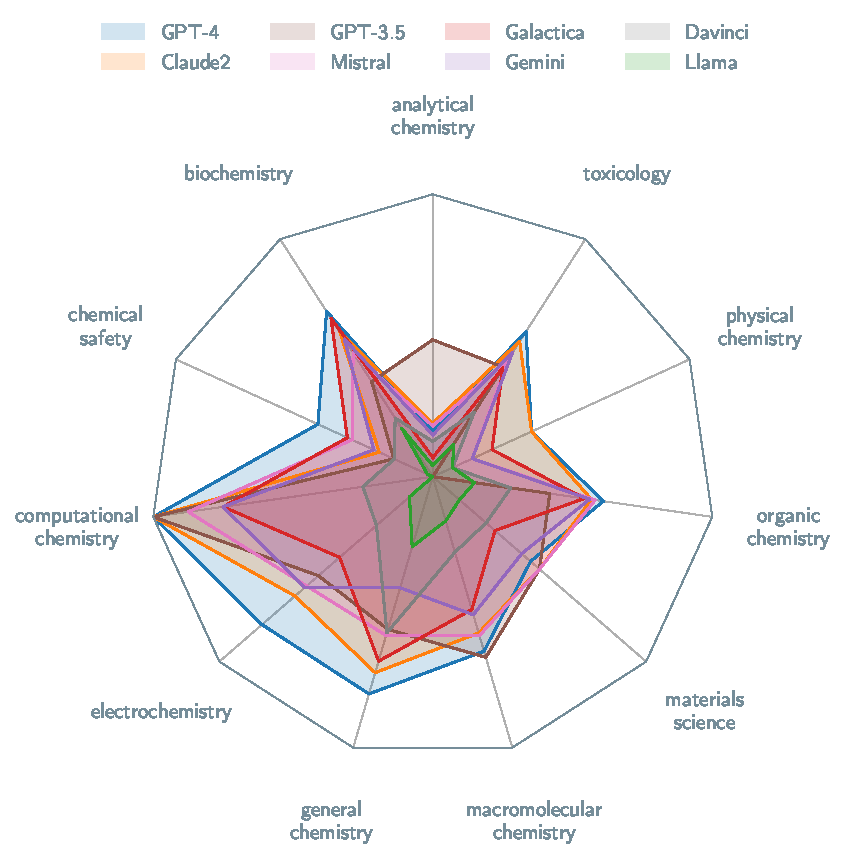
\includegraphics{figures/chem-bench-completely-correct-per-topic.pdf}
    \caption{Caption}
    \label{fig:enter-label}
\end{figure}


\begin{figure}
    \centering
    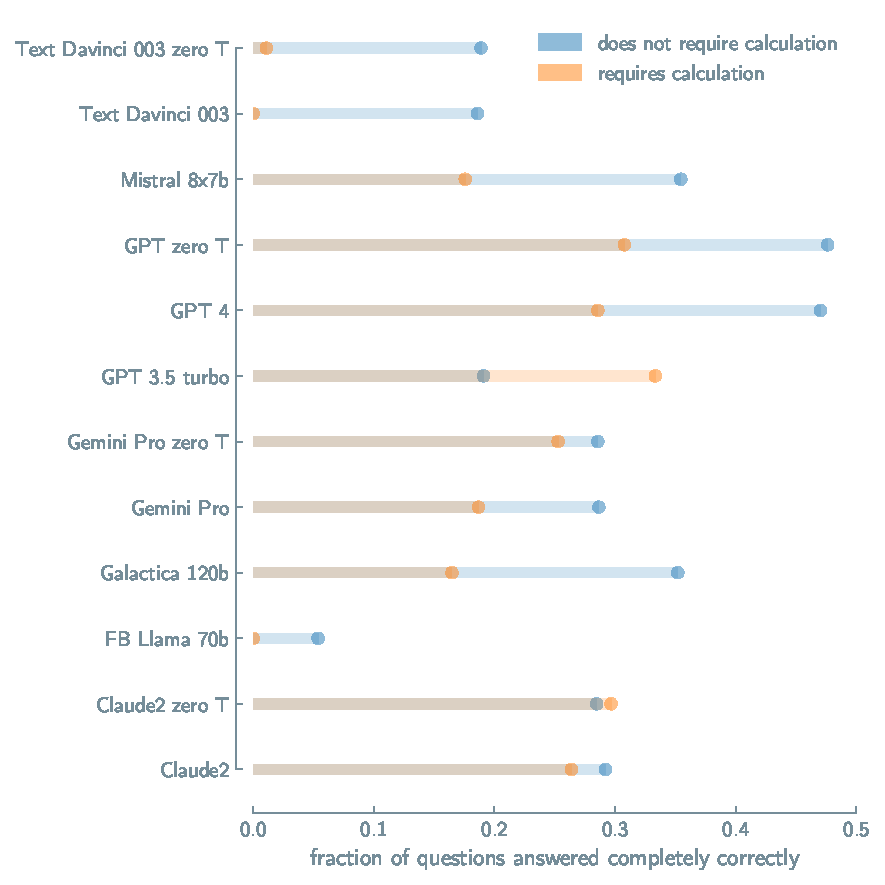
\includegraphics{figures/chem-bench-completley-correct-calculation-vs-no-calculation.pdf}
    \caption{Caption}
    \label{fig:enter-label}
\end{figure}

% \subsubsection{Triggering of safety filters}

\section{Conclusions}

\subsection{Future work}
- Advanced prompting techniques such as CoT and test time strategies 

- More advanced systems with chemnistry specific tools 

- More systematic human baseline: Ask people to come in, do not allow to skip questions

\section{Methods}

\subsection{Curation workflow} \label{sec:curation}
% ToDo: we should not call the first item in the figure curation 
For our dataset we curated questions from existing exams, but also programatically created new questions. Questions were added via Pull Requests on our GitHub repository and only merged into the main collection after passing manual review.

To ensure that the questions do not enter a training dataset we use the canary string of the Big Bench project. This requires that \Gls{llm} developers filter their training dataset for this canary string.  

\begin{figure}
    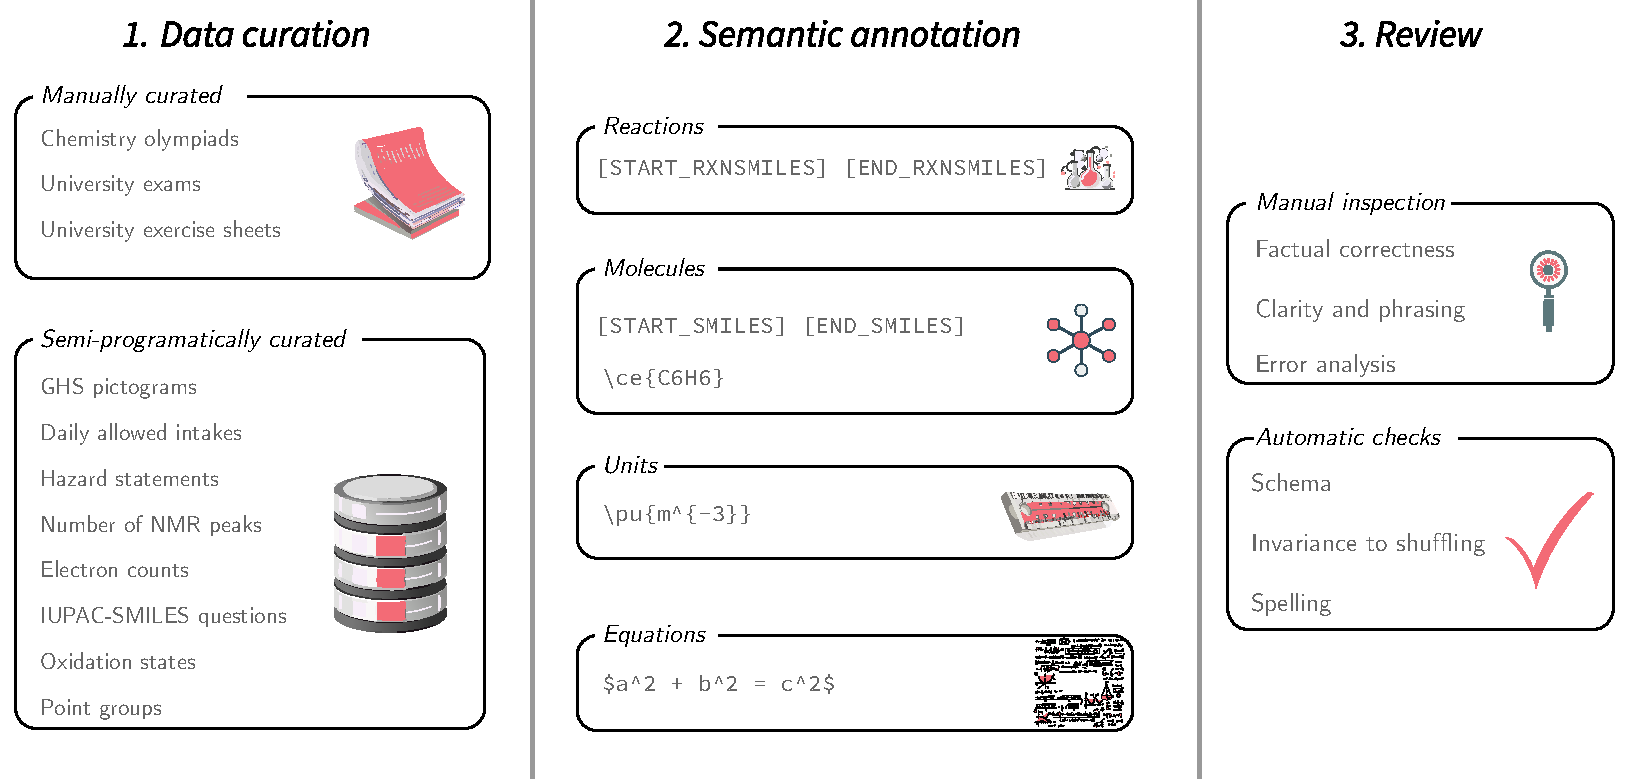
\includegraphics[width=\textwidth]{figures/chem-bench.pdf}
        \caption{\textbf{Data curation workflow}.}
\end{figure}

\paragraph{Manually curated questions}

\paragraph{Semi-programatically generated questions}

\subparagraph{Oxidation states}

\subparagraph{Electron counts}

\paragraph{Programatically generated questions} 
\subparagraph{Number of NMR peaks} To generate tasks about the number of NMR peaks, we randomly sampled SMILES from the ZINC dataset and then used OpenChemLib\cite{openchemlib} to compute the number of diasterotopically distinct hydrogen atoms. 

\subparagraph{GHS classification}

\subparagraph{Hazard statements}

\subparagraph{Number of isomers}


\subsection{Model evaluation workflow}

\paragraph{Prompting}

\paragraph{Parsing}
Our parsing workflow is, by default, multistep and primarily based on regular expressions. 
In the case of instruction-tuned models we first attempt to identify the \texttt{[ANSWER][\textbackslash ANSWER]} environment we prompt the model to report the answer in. 
In the case of completion models, this step is skipped. From there, we attempt to extract the relevant enumeration letters (for multiple-choice questions) or numbers. 
In the case of numbers, our regular expression was engineered to be able to deal with various forms of scientific notation. 
As initial tests indicated that models sometimes return integers in the form of words, e.g. \enquote{one} instead of \enquote{1}, we also implemented a word-to-number conversion. 
In case these hard-coded parsing steps fail, we fall back to using a \gls{llm}, e.g. Claude-2, to parse the completion. 
The frequency of this fallback being triggered was very different for different models (see XX). 
Manual verification (see \Cref{sec:manually-verified-parsing}) indicates that this \gls{llm}-based parsing is not a relevant error source.

\paragraph{Models}


\subsection{Human baseline}

\paragraph{App} To facilitate the collection of responses, we developed a responsive web application in Typescript using the Next.js\cite{nextjs} app router framework. 
This application handles serving the user interface as well as exposes various \gls{rest} \glspl{api} for relevant operations. 
We utilize a MySQL\cite{mysql} database and Prisma \gls{orm}\cite{prisma} for efficient database management. 
The web application is styled with Tailwind CSS\cite{tailwindcss} using the shadcn/ui component library and uses NextAuth\cite{nextauth} for easy and secure user authentication and postMark for sending Emails.
The application is hosted on the Vercel web hosting platform. 

\paragraph{Question selection}
Since we anticipated that we will not be able to collect enough responses for every question to allow for a meaningful statistical analysis, we decided on showing a relevant subset of all questions to the human scorers. 
For selecting the subset, we decided on addressing two questions: 
\begin{itemize}
    \item Are the questions for which the models scored poorly just too difficult or unanswerable? 
    \item Are there areas in which the performance of humans is very different from the ones of the models? 
\end{itemize}
To answer the first question we selected X questions that all \glspl{llm} (model names) from an initial scoring round did not answer correctly. 
From those we picked X diverse one using greedy MaxMin sampling on the embeddings on the questions computed using BART (see below). 


\paragraph{Study design} 
For our initial study we wanted to maximize the response rate given our available resources. For this reason, we did not opt for a highly controlled study setting. That is, while users were prompted to not use external tools other than a calculator and to not consult with other humans, we do not have any way to verify that the participants complied with those rules. Note that users were also allowed to skip questions.


\subsection{Classification of questions into topics} \label{sec:meth-topic} When curating our dataset we systematically recorded keywords and sources. 
To allow for analysis of the model performance as a function of the topic, we leverage this information together with sequence classification models. For questions which can easily be assigned to a topic based on the source (e.g., number of NMR peaks, chemical compatibility, toxicology exam questions) we use this information to make the assignment. For the remaining ones, e.g., from chemistry olympiad questions, we use zero-short sequence classification\cite{zeroshotsequence} using the BART model\cite{bart, FacebookBART}, which our preliminary analysis found to be more robust than topic modeling based on embeddings from OpenAI's \texttt{ada} model or Cohere's \texttt{Cohembed-english-v3.0} model. 




\section*{Data and code availability} 

\section*{Acknowledgements}
This work was supported by the Carl Zeiss Foundation and a \enquote{Talent Fund} of the \enquote{Life} profile line of the Friedrich Schiller University Jena.
We also want to acknowledge access to the HPC cluster of Stability.AI.

\section*{Conflicts of interest}
K.M.J.\ is a paid consultant for OpenAI. M.P.\ is employee of Stability.ai and A.M.\ and N.A.\ are paid contractors of Stability.ai.

\section*{Author contributions}
%Conceptualization
%Data curation
%Formal analysis - Application of statistical, mathematical, computational, or other formal techniques to analyse or synthesize study data.
%Funding acquisition
%Investigation - Conducting a research and investigation process, specifically performing the experiments, or data/evidence collection.
%Methodology
%Project administration
%Resources
%Software
%Supervision
%Validation
%Visualization
%Writing -- original draft
%Writing -- review & editing

\credit{Nawaf~Alampara}{0,1,1,0,1,0,0,0,1,0,0,0,0,0}
\credit{Adrian~Mirza}{0,1,1,0,1,0,0,0,1,0,0,0,0,0}
\credit{Sreekanth~Kunchapu}{0,1,0,0,1,0,0,0,0,0,0,0,0,0}
\credit{Tanya~Gupta}{0,1,0,0,1,0,0,0,0,0,0,0,0,0}
\credit{Jakob~Meyer}{0,1,0,0,0,0,0,0,0,0,0,0,0,0}
\credit{Michael Ringleb}{0,1,0,0,0,0,0,0,0,0,0,0,0,0}
\credit{Maximilian Greiner}{0,1,0,0,0,0,0,0,0,0,0,0,0,0}
\credit{Yannik Köster}{0,1,0,0,0,0,0,0,0,0,0,0,0,0}
\credit{Jan Peschel}{0,1,0,0,0,0,0,0,0,0,0,0,0,0}
\credit{Amir Elahi}{0,1,0,0,0,0,0,0,0,0,0,0,0,0}
\credit{Dinga Wonanke}{0,1,0,0,0,0,0,0,0,0,0,0,0,0}
\credit{Juliane Eberhardt}{0,1,0,0,0,0,0,0,0,0,0,0,0,0}
\credit{Christina Glaubitz}{0,1,0,0,0,0,0,0,0,0,0,0,0,0}
\credit{Mara~Wilhemli}{0,1,0,0,1,0,0,0,0,0,0,0,0,0}
\credit{Macjonathan~Oreke}{0,1,0,0,1,0,0,0,0,0,0,0,0,0}
\credit{Benedict~Emoekabu}{0,1,0,0,1,0,0,0,0,0,0,0,0,0}
\credit{Michael~Pieler}{1,0,0,0,0,0,0,0,0,0,0,0,a0,0}
\credit{Aswanth~Krishnan}{0,0,0,0,0,0,0,0,1,0,0,0,0,0}
\credit{Philippe~Schwaller}{1,1,0,1,1,0,0,0,0,1,0,0,0,0}
\credit{Kevin Maik Jablonka}{1,1,1,1,1,1,1,1,1,1,1,1,1,1}

% \insertcredits

\bibliography{references}

% \appendix

\subsection{Parsing verification} \label{sec:manually-verified-parsing}
For validating the parsing workflow, we randomly sampled four questions per topic and manually verified that the completions of the model were parsed correctly. 

\begin{table}
    \centering
    \begin{tabularx}{\textwidth}{XXXXXXXXXXXX}
        \toprule
        model & general chemistry & electrochemistry & computational chemistry & chemical safety & biochemistry & analytical chemistry & toxicology & physical chemistry & organic chemistry & materials science & macromolecular chemistry \\ 

        \bottomrule
    \end{tabularx}
\end{table}


\subsection{Human baseline}

\begin{figure}
    \centering 
    \includegraphics{figures/human_timing.pdf}
    \script{analyze_human_data.py}
    \label{fig:human_timing}
\end{figure}

\end{document}  
